% ============================================================
% Question Bank: ch06-03 Drawing Geometric Figures (Modified)
% Topic Title: Drawing Geometric Figures with Justification and Technology
% CCSS: 7.G.A.2 (Modified for Indiana)
% Questions: 27 (15 MC + 6 SA + 6 Graphical)
% ============================================================

% --- Multiple Choice Questions (15) ---

\begin{practiceQuestion}{m-6-3-q01}{mc}
\begin{questionText}
A student uses a protractor to draw an angle of $135°$. Which best describes this angle?
\end{questionText}
\choiceA{Acute angle}
\choiceB{Right angle}
\choiceC{Obtuse angle}
\choiceD{Straight angle}
\correctAnswer{C}
\explanation{An obtuse angle measures more than $90°$ but less than $180°$. Since $135°$ is between $90°$ and $180°$, it is obtuse.}
\end{practiceQuestion}

\begin{practiceQuestion}{m-6-3-q02}{mc}
\begin{questionText}
Maya wants to draw a rectangle with length $7$ cm and width $4$ cm. Which tools would best help her draw accurate right angles?
\end{questionText}
\choiceA{Ruler only}
\choiceB{Protractor only}
\choiceC{Ruler and protractor}
\choiceD{Compass only}
\correctAnswer{C}
\explanation{A rectangle requires precise side lengths (measured with a ruler) and $90°$ angles at each corner (measured with a protractor). Both tools are needed for accuracy.}
\end{practiceQuestion}

\begin{practiceQuestion}{m-6-3-q03}{mc}
\begin{questionText}
A geometry software program constructs a regular hexagon. How many sides does the hexagon have, and what is the measure of each interior angle?
\end{questionText}
\choiceA{$5$ sides, $108°$}
\choiceB{$6$ sides, $120°$}
\choiceC{$6$ sides, $135°$}
\choiceD{$8$ sides, $135°$}
\correctAnswer{B}
\explanation{A regular hexagon has $6$ sides. Each interior angle $= \frac{(6-2) \times 180°}{6} = \frac{720°}{6} = 120°$.}
\end{practiceQuestion}

\begin{practiceQuestion}{m-6-3-q04}{mc}
\begin{questionText}
Carlos wants to construct a triangle with angles $60°$, $60°$, and $60°$ using a straightedge and compass. What type of triangle will he construct?
\end{questionText}
\choiceA{Scalene}
\choiceB{Isosceles}
\choiceC{Equilateral}
\choiceD{Right}
\correctAnswer{C}
\explanation{A triangle with three $60°$ angles is equilateral. All three sides are equal, and a compass-and-straightedge construction confirms this by stepping off equal arc lengths.}
\end{practiceQuestion}

\begin{practiceQuestion}{m-6-3-q05}{mc}
\begin{questionText}
A student draws a quadrilateral with exactly one pair of parallel sides. What type of quadrilateral did she draw?
\end{questionText}
\choiceA{Rectangle}
\choiceB{Square}
\choiceC{Parallelogram}
\choiceD{Trapezoid}
\correctAnswer{D}
\explanation{A trapezoid is defined as a quadrilateral with exactly one pair of parallel sides. Rectangles, squares, and parallelograms all have two pairs of parallel sides.}
\end{practiceQuestion}

\begin{practiceQuestion}{m-6-3-q06}{mc}
\begin{questionText}
Using dynamic geometry software, Aisha drags a vertex of a triangle and notices the angle sum always stays at $180°$. What geometric principle does this demonstrate?
\end{questionText}
\choiceA{The exterior angle theorem}
\choiceB{The triangle angle sum theorem}
\choiceC{The Pythagorean theorem}
\choiceD{The triangle inequality theorem}
\correctAnswer{B}
\explanation{The triangle angle sum theorem states that the interior angles of any triangle always add up to $180°$. Dynamic software confirms this by allowing exploration as vertices move.}
\end{practiceQuestion}

\begin{practiceQuestion}{m-6-3-q07}{mc}
\begin{questionText}
To draw a parallelogram, which set of conditions is sufficient?
\end{questionText}
\choiceA{Four sides of equal length}
\choiceB{Two pairs of parallel sides with given lengths and one angle}
\choiceC{One pair of parallel sides only}
\choiceD{Four right angles only}
\correctAnswer{B}
\explanation{Two pairs of parallel sides with their lengths and at least one angle fully determine a parallelogram. Knowing the side lengths and one angle lets you compute the other angles and construct the shape.}
\end{practiceQuestion}

\begin{practiceQuestion}{m-6-3-q08}{mc}
\begin{questionText}
Ben uses a compass set to a radius of $4$ cm. He draws a circle and then marks off equal arcs around the circle to construct a regular polygon. If he marks $5$ equally spaced arcs, which polygon does he construct?
\end{questionText}
\choiceA{Square}
\choiceB{Pentagon}
\choiceC{Hexagon}
\choiceD{Octagon}
\correctAnswer{B}
\explanation{Marking $5$ equally spaced points on a circle and connecting consecutive points creates a regular pentagon with $5$ equal sides.}
\end{practiceQuestion}

\begin{practiceQuestion}{m-6-3-q09}{mc}
\begin{questionText}
A student justifies that a drawn quadrilateral is a rectangle by measuring all four angles. What must each angle measure?
\end{questionText}
\choiceA{$60°$}
\choiceB{$90°$}
\choiceC{$120°$}
\choiceD{$180°$}
\correctAnswer{B}
\explanation{A rectangle has four right angles. To justify that a quadrilateral is a rectangle, each angle must measure exactly $90°$.}
\end{practiceQuestion}

\begin{practiceQuestion}{m-6-3-q10}{mc}
\begin{questionText}
Using geometry software, Layla constructs a triangle with sides $5$ cm, $5$ cm, and $5$ cm. She measures each angle and finds they are all equal. What does the software confirm about this triangle?
\end{questionText}
\choiceA{It is a right triangle}
\choiceB{It is an isosceles triangle but not equilateral}
\choiceC{It is equilateral, and each angle is $60°$}
\choiceD{It is obtuse}
\correctAnswer{C}
\explanation{A triangle with three equal sides is equilateral. An equilateral triangle also has three equal angles, each measuring $\frac{180°}{3} = 60°$.}
\end{practiceQuestion}

\begin{practiceQuestion}{m-6-3-q11}{mc}
\begin{questionText}
To construct a perpendicular bisector of a segment using a compass and straightedge, which step comes first?
\end{questionText}
\choiceA{Draw the midpoint using a ruler}
\choiceB{Place the compass on one endpoint and draw an arc above and below the segment}
\choiceC{Measure the segment with a protractor}
\choiceD{Draw a line parallel to the segment}
\correctAnswer{B}
\explanation{The first step of the perpendicular bisector construction is to set the compass wider than half the segment, then place it on one endpoint and draw arcs above and below the segment. Repeating from the other endpoint creates intersection points.}
\end{practiceQuestion}

\begin{practiceQuestion}{m-6-3-q12}{mc}
\begin{questionText}
Ethan draws a rhombus with side length $6$ cm and one angle of $70°$. What is the measure of the angle adjacent to the $70°$ angle?
\end{questionText}
\choiceA{$70°$}
\choiceB{$90°$}
\choiceC{$110°$}
\choiceD{$140°$}
\correctAnswer{C}
\explanation{In a rhombus, consecutive angles are supplementary: $180° - 70° = 110°$. This follows because opposite sides of a rhombus are parallel, making consecutive angles co-interior angles.}
\end{practiceQuestion}

\begin{practiceQuestion}{m-6-3-q13}{mc}
\begin{questionText}
Sofia uses dynamic geometry software to draw a circle and then inscribes a regular hexagon inside it. If the radius of the circle is $5$ cm, what is the side length of the hexagon?
\end{questionText}
\choiceA{$2.5$ cm}
\choiceB{$5$ cm}
\choiceC{$7.5$ cm}
\choiceD{$10$ cm}
\correctAnswer{B}
\explanation{A key property of a regular hexagon inscribed in a circle is that each side length equals the radius of the circle. So the side length is $5$ cm.}
\end{practiceQuestion}

\begin{practiceQuestion}{m-6-3-q14}{mc}
\begin{questionText}
A student is asked to draw a quadrilateral with two pairs of equal sides where the equal sides are adjacent (not opposite). What shape is this?
\end{questionText}
\choiceA{Rectangle}
\choiceB{Parallelogram}
\choiceC{Kite}
\choiceD{Trapezoid}
\correctAnswer{C}
\explanation{A kite has two distinct pairs of consecutive (adjacent) sides that are equal in length. This distinguishes it from a parallelogram, where equal sides are opposite.}
\end{practiceQuestion}

\begin{practiceQuestion}{m-6-3-q15}{mc}
\begin{questionText}
Which justification correctly explains why the sum of the interior angles of any quadrilateral is $360°$?
\end{questionText}
\choiceA{A quadrilateral has four sides, and $4 \times 90 = 360$}
\choiceB{A quadrilateral can be divided into two triangles, each with an angle sum of $180°$}
\choiceC{A quadrilateral is half of a circle, and a full circle is $360°$}
\choiceD{All quadrilaterals have four right angles}
\correctAnswer{B}
\explanation{Drawing a diagonal in any quadrilateral divides it into two triangles. Since each triangle has an angle sum of $180°$, the quadrilateral's angle sum is $2 \times 180° = 360°$.}
\end{practiceQuestion}

% --- Short Answer Questions (6) ---

\begin{practiceQuestion}{m-6-3-q16}{sa}
\begin{questionText}
Using a ruler and protractor, describe the steps to draw a triangle with sides $6$ cm and $8$ cm and an included angle of $50°$.
\end{questionText}
\correctAnswer{Draw a $6$-cm segment, measure a $50°$ angle at one end, draw an $8$-cm ray at that angle, and connect the endpoints.}
\explanation{This is the SAS construction. Step 1: Draw one side ($6$ cm) with a ruler. Step 2: Use a protractor to measure a $50°$ angle at one endpoint. Step 3: Draw the second side ($8$ cm) along that ray. Step 4: Connect the free endpoints to complete the triangle.}
\end{practiceQuestion}

\begin{practiceQuestion}{m-6-3-q17}{sa}
\begin{questionText}
A regular octagon has $8$ sides. What is the measure of each interior angle?
\end{questionText}
\correctAnswer{$135°$}
\explanation{Interior angle of a regular polygon $= \frac{(n - 2) \times 180°}{n}$. For $n = 8$: $\frac{(8-2) \times 180°}{8} = \frac{1080°}{8} = 135°$.}
\end{practiceQuestion}

\begin{practiceQuestion}{m-6-3-q18}{sa}
\begin{questionText}
Explain why a compass-and-straightedge construction of an equilateral triangle works when you set the compass to the length of one side and draw arcs from both endpoints.
\end{questionText}
\correctAnswer{The arcs have the same radius as the base, so the intersection point is equidistant from both endpoints, making all three sides equal.}
\explanation{Both arcs have a radius equal to the base length. Their intersection point is exactly one side length from each endpoint, creating three equal sides. This guarantees an equilateral triangle by the SSS congruence condition.}
\end{practiceQuestion}

\begin{practiceQuestion}{m-6-3-q19}{sa}
\begin{questionText}
Using geometry software, Kevin draws a parallelogram with one angle of $65°$. What are the measures of all four interior angles?
\end{questionText}
\correctAnswer{$65°$, $115°$, $65°$, $115°$}
\explanation{In a parallelogram, opposite angles are equal and consecutive angles are supplementary. So the angles are $65°$, $180° - 65° = 115°$, $65°$, and $115°$.}
\end{practiceQuestion}

\begin{practiceQuestion}{m-6-3-q20}{sa}
\begin{questionText}
Justify why it is impossible to draw a triangle with angles $90°$, $100°$, and $50°$.
\end{questionText}
\correctAnswer{The angles sum to $240°$, which exceeds $180°$. A triangle's angles must sum to exactly $180°$.}
\explanation{By the triangle angle sum theorem, the three interior angles must total $180°$. Here $90 + 100 + 50 = 240 \neq 180$, so these angles cannot form a triangle.}
\end{practiceQuestion}

\begin{practiceQuestion}{m-6-3-q21}{sa}
\begin{questionText}
A student uses a protractor to draw angles of $70°$ and $55°$ at the two ends of a $10$-cm line segment, then extends the rays until they intersect. What is the third angle of the resulting triangle, and what construction condition does this represent?
\end{questionText}
\correctAnswer{$55°$; ASA (Angle-Side-Angle)}
\explanation{The third angle is $180° - 70° - 55° = 55°$. The student used two angles and the included side, which is the ASA condition. ASA produces a unique triangle.}
\end{practiceQuestion}

% --- Graphical MC Questions (3) ---

\begin{practiceQuestion}{m-6-3-q22}{gmc}
\begin{questionText}
The figure below shows a compass-and-straightedge construction. Two arcs from endpoints $A$ and $B$ of a segment intersect at point $C$. If $AC = BC = AB$, what shape is triangle $ABC$?

\begin{center}
\begin{tikzpicture}[scale=0.8]
  \coordinate (A) at (0,0);
  \coordinate (B) at (4,0);
  \coordinate (C) at (2,3.46);
  \draw[thick] (A) -- (B);
  % Arcs
  \draw[thick,funBlue,dashed] (0,0) arc[start angle=-30,end angle=90,radius=4];
  \draw[thick,funRed,dashed] (4,0) arc[start angle=210,end angle=90,radius=4];
  % Triangle
  \draw[thick] (A) -- (C) -- (B);
  \fill (A) circle (2pt) node[below] {$A$};
  \fill (B) circle (2pt) node[below] {$B$};
  \fill (C) circle (2pt) node[above] {$C$};
\end{tikzpicture}
\end{center}
\end{questionText}
\choiceA{Right triangle}
\choiceB{Isosceles triangle}
\choiceC{Equilateral triangle}
\choiceD{Scalene triangle}
\correctAnswer{C}
\explanation{Since $AC = BC = AB$, all three sides are equal, making the triangle equilateral. Each angle measures $60°$. The arcs ensure the third vertex is equidistant from both endpoints.}
\end{practiceQuestion}

\begin{practiceQuestion}{m-6-3-q23}{gmc}
\begin{questionText}
The diagram shows a square with a diagonal drawn. The diagonal divides the square into two triangles. What is the measure of each non-right angle in the triangles?

\begin{center}
\begin{tikzpicture}[scale=0.8]
  \draw[thick,fill=funGreen!10] (0,0) rectangle (4,4);
  \draw[thick,funRed] (0,0) -- (4,4);
  % Right angle marks
  \draw (0.3,0) -- (0.3,0.3) -- (0,0.3);
  \draw (3.7,0) -- (3.7,0.3) -- (4,0.3);
  \draw (0,3.7) -- (0.3,3.7) -- (0.3,4);
  \draw (3.7,4) -- (3.7,3.7) -- (4,3.7);
  % Labels
  \node at (1,0.6) {$?$};
  \node at (3,3.4) {$?$};
  \node at (0.6,3.4) {$90°$};
\end{tikzpicture}
\end{center}
\end{questionText}
\choiceA{$30°$}
\choiceB{$45°$}
\choiceC{$60°$}
\choiceD{$90°$}
\correctAnswer{B}
\explanation{A diagonal of a square creates two right isosceles triangles. Each triangle has one $90°$ angle (the corner of the square). The other two angles are equal and sum to $90°$: $\frac{90°}{2} = 45°$ each.}
\end{practiceQuestion}

\begin{practiceQuestion}{m-6-3-q24}{gmc}
\begin{questionText}
The figure shows a kite $ABCD$ with the given side lengths. What is the perimeter of the kite?

\begin{center}
\begin{tikzpicture}[scale=0.7]
  \coordinate (A) at (0,0);
  \coordinate (B) at (2,3);
  \coordinate (C) at (0,5);
  \coordinate (D) at (-2,3);
  \draw[thick,fill=funBlue!10] (A) -- (B) -- (C) -- (D) -- cycle;
  \node[below] at (0,0) {$A$};
  \node[right] at (2,3) {$B$};
  \node[above] at (0,5) {$C$};
  \node[left] at (-2,3) {$D$};
  \node[right] at (1.2,1.3) {$5$ cm};
  \node[right] at (1.2,4.2) {$4$ cm};
  \node[left] at (-1.2,4.2) {$4$ cm};
  \node[left] at (-1.2,1.3) {$5$ cm};
\end{tikzpicture}
\end{center}
\end{questionText}
\choiceA{$9$ cm}
\choiceB{$13$ cm}
\choiceC{$18$ cm}
\choiceD{$20$ cm}
\correctAnswer{C}
\explanation{A kite has two pairs of adjacent equal sides. The perimeter is $5 + 5 + 4 + 4 = 18$ cm.}
\end{practiceQuestion}

% --- Graphical SA Questions (3) ---

\begin{practiceQuestion}{m-6-3-q25}{gsa}
\begin{questionText}
The diagram shows the first two steps of constructing a perpendicular bisector of segment $\overline{AB}$. Describe the remaining steps and justify why the construction works.

\begin{center}
\begin{tikzpicture}[scale=0.7]
  \coordinate (A) at (0,0);
  \coordinate (B) at (6,0);
  \draw[thick] (A) -- (B);
  \fill (A) circle (2pt) node[below] {$A$};
  \fill (B) circle (2pt) node[below] {$B$};
  % Arcs from A
  \draw[thick,funBlue,dashed] (0,0) ++(60:4) arc[start angle=60,end angle=-60,radius=4];
  % Arcs from B
  \draw[thick,funRed,dashed] (6,0) ++(120:4) arc[start angle=120,end angle=240,radius=4];
  % Intersection points
  \coordinate (P) at (3,2.65);
  \coordinate (Q) at (3,-2.65);
  \fill (P) circle (2pt) node[above right] {$P$};
  \fill (Q) circle (2pt) node[below right] {$Q$};
\end{tikzpicture}
\end{center}
\end{questionText}
\correctAnswer{Draw a straight line through $P$ and $Q$. This line is the perpendicular bisector because $P$ and $Q$ are equidistant from $A$ and $B$.}
\explanation{After drawing arcs from both endpoints with the same radius, the intersection points $P$ and $Q$ are each equidistant from $A$ and $B$. The line through $P$ and $Q$ passes through the midpoint of $\overline{AB}$ at a $90°$ angle, forming the perpendicular bisector.}
\end{practiceQuestion}

\begin{practiceQuestion}{m-6-3-q26}{gsa}
\begin{questionText}
The incomplete quadrilateral below has three vertices plotted. Place the fourth vertex $D$ so that $ABCD$ forms a parallelogram. Justify your answer.

\begin{center}
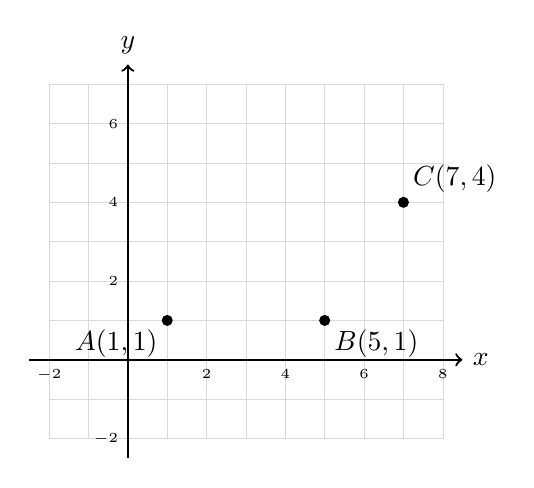
\begin{tikzpicture}[scale=0.5]
  \draw[help lines,gray!30] (-2,-2) grid (8,7);
  \draw[thick,->] (-2.5,0) -- (8.5,0) node[right] {$x$};
  \draw[thick,->] (0,-2.5) -- (0,7.5) node[above] {$y$};
  \foreach \x in {-2,2,4,6,8} \node[below] at (\x,0) {\tiny $\x$};
  \foreach \y in {-2,2,4,6} \node[left] at (0,\y) {\tiny $\y$};
  \fill (1,1) circle (4pt) node[below left] {$A(1,1)$};
  \fill (5,1) circle (4pt) node[below right] {$B(5,1)$};
  \fill (7,4) circle (4pt) node[above right] {$C(7,4)$};
\end{tikzpicture}
\end{center}
\end{questionText}
\correctAnswer{$D(3, 4)$}
\explanation{In a parallelogram, opposite sides are parallel and equal. From $A$ to $B$: right $4$, up $0$. For $DC$ to be parallel and equal: $D$ must be $4$ units left of $C$: $(7 - 4, 4) = (3, 4)$. Verify: $\overrightarrow{AD} = (2, 3)$ and $\overrightarrow{BC} = (2, 3)$, so $AD \parallel BC$ and $AD = BC$.}
\end{practiceQuestion}

\begin{practiceQuestion}{m-6-3-q27}{gsa}
\begin{questionText}
Using the diagram below, determine the sum of the interior angles of the pentagon by dividing it into triangles. Show how many triangles are formed and calculate the total angle sum.

\begin{center}
\begin{tikzpicture}[scale=0.8]
  \coordinate (A) at (0,1);
  \coordinate (B) at (2,0);
  \coordinate (C) at (4,0.5);
  \coordinate (D) at (4,3);
  \coordinate (E) at (1,3.5);
  \draw[thick,fill=funBlue!10] (A) -- (B) -- (C) -- (D) -- (E) -- cycle;
  % Diagonals from vertex A
  \draw[thick,dashed,funRed] (A) -- (C);
  \draw[thick,dashed,funRed] (A) -- (D);
  \node[left] at (A) {$A$};
  \node[below] at (B) {$B$};
  \node[right] at (C) {$C$};
  \node[right] at (D) {$D$};
  \node[above] at (E) {$E$};
  \node at (1.5,0.8) {\small $1$};
  \node at (2.5,1.8) {\small $2$};
  \node at (1.8,2.8) {\small $3$};
\end{tikzpicture}
\end{center}
\end{questionText}
\correctAnswer{$3$ triangles; $540°$}
\explanation{Drawing diagonals from one vertex of a pentagon divides it into $3$ triangles. Each triangle has an angle sum of $180°$. Total: $3 \times 180° = 540°$. In general, an $n$-sided polygon has angle sum $(n - 2) \times 180°$.}
\end{practiceQuestion}
